\documentclass[9pt,twocolumn,twoside,lineno]{pnas-new}
% Use the lineno option to display guide line numbers if required.

\usepackage{float}

\templatetype{pnasresearcharticle} % Choose template 
% {pnasresearcharticle} = Template for a two-column research article
% {pnasmathematics} %= Template for a one-column mathematics article
% {pnasinvited} %= Template for a PNAS invited submission

\setboolean{displaywatermark}{false}

\title{Optimisation of Role Models in unweighted networks}

% Use letters for affiliations, numbers to show equal authorship (if applicable) and to indicate the corresponding author
\author[a]{Aleksander Kaminski}

\affil[a]{Mathematical Institute, University of Oxford}

% Please give the surname of the lead author for the running footer
\leadauthor{Kaminski} 

% Please add here a significance statement to explain the relevance of your work
\significancestatement{The study of networks is a large and blooming field, with possible applications in nearly all fields of science, from map-networks for use in navigation to social-networks in epidemiology. Of much interest is the 'role-modelling' networks, where the network nodes are partitioned into distinct sets by the function they play in the network. For example, a large neural network could be partitioned into 3 groups, of inter-, motor, and sensory neurons. Methods for calculating these partitions rely on the optimisation of discrete functions. Two such methods are analysed in this article.}

% Please include corresponding author, author contribution and author declaration information
\correspondingauthor{\textsuperscript{1}To whom correspondence should be addressed. E-mail: aleksander.kaminski@oriel.ox.ac.uk}

\begin{abstract}
We present, implement, and analyse gradient descent and simualted annealing as applied to the optimisation of equation (6) as presented in "Reichardt J, White DR (2007) Role models for complex networks". We find that for certain sizes block structures, this equation doesn't correctly determine the block-image and has tendencies to miss edges. We analyse (6) to find an efficient $O(N)$ way to update state cost when moving to neighbouring states. With this we found that both algorithms perform well for small $N \approx 50$ networks and outline the difficulting in choosing the correct inital parameters for both algorithms. We then apply our implementations to present the block structure of an empirical network.   
\end{abstract}

\dates{This manuscript was compiled on \today}
\doi{\url{www.pnas.org/cgi/doi/10.1073/pnas.XXXXXXXXXX}}

\begin{document}

\maketitle
\thispagestyle{firststyle}
\ifthenelse{\boolean{shortarticle}}{\ifthenelse{\boolean{singlecolumn}}{\abscontentformatted}{\abscontent}}{}

% If your first paragraph (i.e. with the \dropcap) contains a list environment (quote, quotation, theorem, definition, enumerate, itemize...), the line after the list may have some extra indentation. If this is the case, add \parshape=0 to the end of the list environment. 
\dropcap{M}any algorithms that deal with network partitioning rely on the optimisation of a cost function, $Q$, of the partitions. The number of such partitions is $O(M^N)$ with the number of nodes, $N$, and partitions, $M$, of a network. This makes the problem of finding the exact maximum using brute-force searches intractible. Thus, for large $N$ networks, more intelligent approaches have to be used to optimise such functions. In this article we explore the usage of gradient descent (GD) and simulated annealing (SA) algorithms. Both of these algorithms rely on the exploration of a state-space, and we show how both can be viewed as graph traversals of such a state-space. 

\subsection*{State-space}
A partition of the nodes of a network can be thought of as an $N$-vector, the entries of which take the values  $1, 2, \ldots, M$. We can define two states $\sigma_1$ and  $\sigma_2$ to be neighbours if $\sigma_1$ and $\sigma_2$ differ only in 1 entry. More precisely, there is some  $i$ such that $\sigma_1^i \neq \sigma_2^i$ and for all $j \neq i$, $\sigma_1^j = \sigma_2^j$. Using this notion of neighbourhood, we can construct a state-graph, where two states are connected by an edge if they are neighbours. For the purposes of optimisation we impose one other constraint on the state-graph. Namely, for all states $\sigma$ it must be true that, for all roles $m \in [1, \ldots, M]$, there is at least one $i \in [1, \ldots, N]$ such that $\sigma^i = m$. In other words, this means that all states have at least node in each role. The choice of neighbourhood of states greatly affects the performance of both of the algorithms considered, as both optimise locally. 

\subsection*{Gradient Descent}  
The gradient descent algorithm implemented here is inspired by gradient descent on continuous functions. We genralise by considering the differences of cost between neighbouring states, rather than derivatives. For a simple neighbourhood like we're considering, every neighbouring state is distance $1$ away. Thus, our algorithm reduces to just repeatedly moving to the state which maximises this difference. \\
More formally, let $Q$ be a function of which we want to find a global maximum. Let $\sigma$ be a state. For each neighbouring state $\eta$ to $\sigma$, calculate the difference in cost of changing to the new state $\Delta_{\sigma \to \eta} = Q(\eta) - Q(\sigma)$. Choose the $\eta$ that maximises $\Delta_{\sigma \to \eta}$, which can be done by brute-force. For more complex neighbourhoods, $\frac{\Delta_{\sigma \to \eta}}{d(\sigma, \eta)}$ can be considered. This procedure repeats until for all eta $\Delta_{\sigma \to \eta} \leq 0$. We denote this final state by  $\sigma^*$. One downside to this simple procedure is that it has the tendency to get stuck in local-maxima. To avail this, the algorithm is repeated $R$ times, each time choosing a random inital state state. The state maximising the cost, over many realisations, is chosen as the optimum. $R$ is taken as a parameter. Up to the choice of the inital state, this algorithm is deterministic. 

\subsection*{Simulated Annealing}
Simulated annealing relies on exploring the state-graph in a probablistic manner. Let $Q$ be the function we're maximising, and let  $\sigma$ be the current state.  Let $\eta$ be a \textit{random} neighbor of $\sigma$. We calculate  $\Delta_{\sigma \to \eta}$. If $\Delta_{\sigma \to \eta} \geq 0$ then we accept $\eta$ as the new state. If $\Delta_{\sigma \to \eta} < 0$ then we accept $\eta$ with probability

\begin{align*} 
    P(\sigma \to \eta) = \exp(\frac{\Delta_{\sigma \to \eta}}{T}).  
\end{align*} 
We run this procedure $R_{i}$ times, before adjusting the  $T$ parameter. 
Intuitively we can view -$Q(\sigma)$ as the energy of a state, and  $T$ as a physical temperature. In this picture this procedure is analogous to how real physical systems crystalize into low-energy states. 
The way $T$ is adjusted after iterating is referred to as the annealing schedule. In this article we explore two annealing schedules,  $T_{t+1} = \alpha T_{t}$, and $T = T_{max} * (1 +  t)^{-1}$. We iterate the procedure from some max temperature $T_{max}$ at $t = 0$ to a minimum temperature  $T_{min}$.

\section*{Method}
In this article we focus on maximising a specific quality function, as given by equation 6 in \cite{role_models}. For ease of notation introduce the sets $C_{r} = \{\, i \in [1, N] \,|\, \sigma^i = r\,\}$. Denote by $E$ the number of edges in the network. We make the same choice of convention as in the \cite{role_models}, taking $a_{ij} = 1 - p_{ij}$, $b_{ij} = p_{ij}$ with  $p_{ij} = (k^{out}_i k^{in}_j)/E$. Introducing the matrix $B$, where  $B_{ij} = p_{ij}$ we can write the fraction of edges, as well as the expected fraction of edges between communities r, s as

\begin{align*}
    e_{rs} &= \frac{1}{E}\sum_{i \in C_r, j \in C_s} A_{ij} \numberthis \label{eqn:eRAW}\\
    [e_{rs}] &= \frac{1}{E}\sum_{i \in C_r, j \in C_s} B_{ij} \numberthis \label{eqn:EeRAW}
\end{align*}
which showcases the similarity between these two quantities. Now we can write the quality function of a state as 

\begin{align*}
    Q^*(\sigma) = \frac{1}{2} \sum_{r, s}^M  \mid e_{rs} - [e_{rs}]  \mid \numberthis \label{eqn:co} 
\end{align*} 
A naive implementation of this function for a general state $\sigma$ is  $O(N^2 + M^2) = O(N^2)$ as $N > M$ which gets prohibitively expensive with large  $N$ networks. This can be seen by noticing that we need to compute $e_{rs}$ and  $[e_{rs}]$, which is  $O(N^2)$, and then we need to compute  $Q^*(\sigma)$ which is  $O(M^2)$. We can improve this significantly by noticing that a change from state $\sigma$ to $\eta$ moves a node $i$ from role $I$ to role $F$. If both $r \notin \{I, F\} $ and $s \notin \{I, F\}$ then $e_{rs}$ and $[e_{rs}]$ don't differ between $\sigma$ and $\eta$. This suggests an improvement from $O(M^2)$ to  $O(M)$, but we find that this is even better. One more thing to notice is that any performance improvement we make for $e_{rs}$ is automatically applicable to $[e_{rs}]$, given that they are both functions of the partitions in the same manner. In order to pursue this, we rerwrite \ref{eqn:eRAW} and \ref{eqn:EeRAW} in a different form. Introducing the notation

\begin{align*}
    K^{in}_{i \to r} &= \sum_{j \in C_r, j \neq i} A_{ij} \numberthis \label{eqn:kin} \\
    K^{out}_{i \to r} &= \sum_{j \in C_r, j \neq i}^N A_{ji}. \numberthis \label{eqn:kout}
\end{align*}
Where these quantities represent the in/out degrees of node $i$ into and out of role $r$, respectively. We can also define $[K^{in}_{i \to r}]$ and $[K^{out}_{i \to r}]$ analogously by substituting B for A in the above equations. Now we write \ref{eqn:eRAW} and \ref{eqn:EeRAW} as,  

\begin{align*}
    e_{rs} &= \frac{1}{E}\sum_{i \in C_r} K^{in}_{i \to s} = \frac{1}{E}\sum_{j \in C_s} K^{out}_{j \to r} \numberthis \label{eqn:e} \\
    [e_{rs}] &= \frac{1}{E}\sum_{i \in C_r} [K^{in}_{i \to s}] = \frac{1}{E}\sum_{j \in C_s} [K^{out}_{j \to r}]. \numberthis \label{eqn:Ee} 
\end{align*}
Reusing our previous notatation in moving $i$ from  $I$ to  $F$, we compute the deltas of these new quantities. Let $j$ be any node other than i, omitting any quantities that do not change, we can write the deltas as

\begin{align*}
    K^{in}_{j \to I} &\mapsto K^{in}_{j \to I} - A_{ji} \\
    K^{out}_{j \to I} &\mapsto K^{out}_{j \to I} - A_{ij} \\
    K^{in}_{j \to F} &\to K^{in}_{j \to F} + A_{ji} \\
    K^{out}_{j \to F} &\to K^{out}_{j \to F} + A_{ij}. 
\end{align*}
And analogously for $[K^{in / out}_{j \to s}]$. Now we can use these to calculate the changes to $e_{rs}$. Let $p$ be any role, then

\begin{align*}
    e_{Ip} &\mapsto e_{Ip} - \frac{1}{E}K^{in}_{i \to p} \\ 
    e_{Fp} &\mapsto e_{Fp} + \frac{1}{E}K^{in}_{i \to p} \\
    e_{pI} &\mapsto e_{pI} - \frac{1}{E}K^{out}_{i \to p} \\
    e_{pF} &\mapsto e_{pF} + \frac{1}{E}K^{out}_{i \to p},
\end{align*}
where any updates that appear twice are taken to be performed sequentially (for example $p = I$,  $e_{pI}$ and  $e_{Ip}$ both update  $e_{II}$). The updating of $K^{in}_{j \to r}$ is $O(N)$, and the updating of $e_{rs}$ is $O(M)$. Given that  $M < N$, we have improved the computational complexity of  from  $O(N^2 + M^2)$ to  $O(N + M^3)$. Further, the computation of the cost fuction can be reduced from $O(M^2)$ to $O(M)$, by considering only the changed quanities, but we do not attempt this here. 
\subsection*{Graph analysis}
We analyse our implementation of the SA and GD algorithms by applying them to networks exhibiting block structure. We to this by creating these networks in reverse, starting with some (given) block structure, and creating a network out of this. Usually, the number of roles in such a matrix is given by the matrix dimensions. For example the block-image given by the 3x3 matrix

\begin{align*}
    A^{block} = 
   \begin{pmatrix} 
       1 & 0 & 0 \\
       1 & 0 & 1 \\
       0 & 0 & 1 
   \end{pmatrix} 
\end{align*}
would have 3 roles. In this block-image, nodes 1 and 3 are structurally equivalent, but are still treated as separate roles. This is because we can have a partition of the nodes that have edges from node 2 into two disjoint subsets of nodes that only interact with eachother. Though, one freedom we do have in the determination of a block structure from a matrix is by relabelling nodes. Out of such a block image, we can create a network by treating each block as an Erdős–Rényi graph. We use 3 parameters, $p_{int}$, $p_{ext}$, and $N_{b}$. These satisfy

\begin{align*}
    p_{int} > p_{ext} \numberthis \label{eqn:prob}.
\end{align*}
For each entry $A^{block}_{ij}$, we generate the corresponding adjacency matrix $A_{ij} \in \{0, 1\}^{N_b}\times\{0, 1\}^{N_b}$, where $A_{ij}$ ER with edge probability $p_{int}$ if $A^{block}_{ij}$ and $p_{ext}$ otherwise. Let $E^{block}$ the number of edges of the block matrix. As we want to keep the total number of edges roughly constant, we define a new probability $p_{edge}$ which should satisfy

\begin{align*}
    {N_b}^2 p_{edge} &= E^{block} p_{int} + ({N_b}^2 - E^{block}) p_{ext}  
\end{align*}
and so

\begin{align}
    p_{ext} &= \frac{{N_b}^2 p_{edge} - E^{block} p_{int}}{{N_b}^2 - E^{block}}
\end{align}
also this implies that the minmum value of $p_{int}$ that satisfies \ref{eqn:prob} is $p_{edge}$. For each role we also test how the convergence behaves as we add some variability to the sizes of each block. We do this by adding a unifomly distributed offset to each block size. We call this offset $N_b^o$, so that  the size lies between $N_b - N_b^o$ and $N_b + N_b^o$.


\begin{figure*}%[th]
\centering
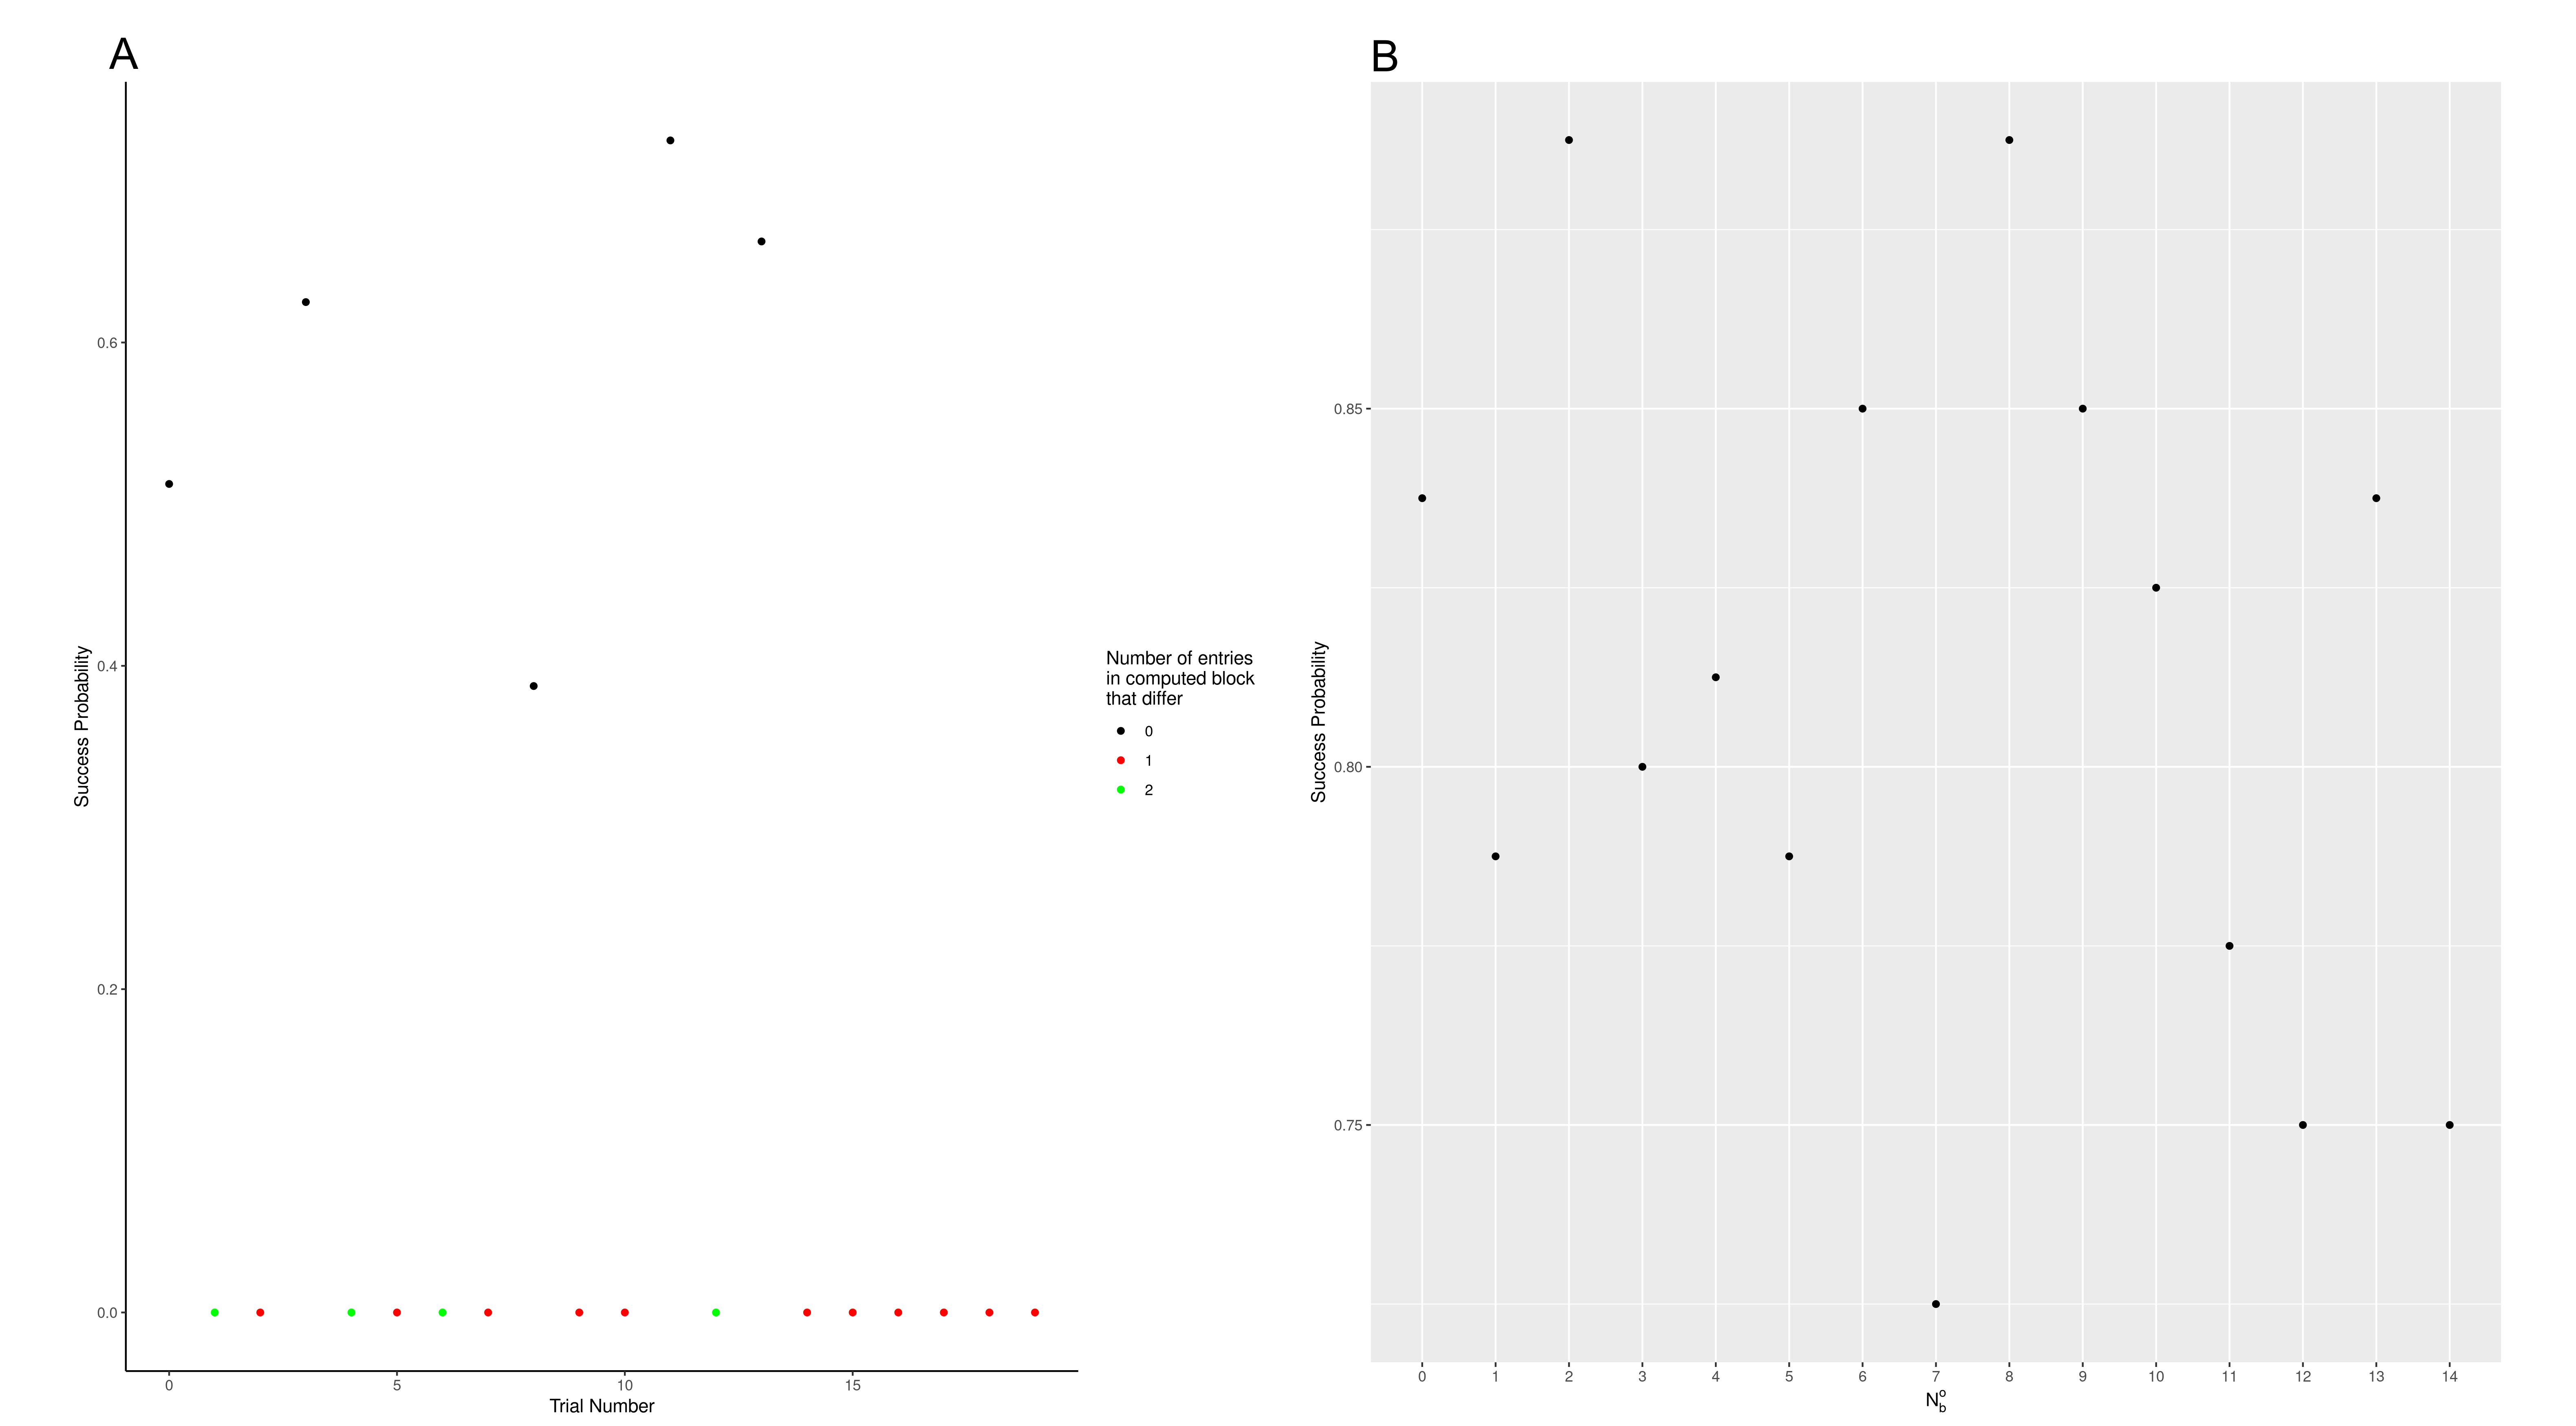
\includegraphics[width=.9\linewidth]{figures/NB_VAR}
\caption{The probability of finding the correct block for graphs with $N_b = 20$ and $N_b^o = 5$ per run of GD, for different values of $P_{int}$, while keeping the number of edges constant. The probability increases rapidly from $0$ to $0.4$ at $P_{int} \approx 0.6$. It keeps increasing until it is roughly constant above $p_{int}$ = 0.8. Another feature of the graph is showing whether the block-image found from the partition maximising \ref{eqn:co} converges to the correct block image, which is found to not be the case for half of the networks considered. }
\label{fig:GD_resolving}
\end{figure*}

\subsection*{Analysis of Gradient Descent}
We analysed the dependence of the gradient descent algorithm on the connectedness of blocks. We started with a block-image of the form. 

\begin{align*}
    A = 
    \begin{pmatrix} 
        0 & 1 & 0 & 0 \\
        0 & 1 & 1 & 0 \\
        0 & 0 & 0 & 1 \\
        1 & 1 & 0 & 0 
    \end{pmatrix} 
\end{align*}

The graph of which can be seen in Fig. \ref{fig:GD_block}. The results of the analysis are presented in Fig. \ref{fig:GD_random_fill}. Of note is that, with $N_b^o > 0$ we get the situation that certain edges become unresolved by the optimisation of \ref{eqn:co}. This is tested further in Fig. \ref{fig:GD_resolving}. We chose a random unresolved network and a random resolved network from those tested and show its adjacency matrix in Fig. \ref{fig:GD_adj}. From this we deduce that the unresolved network has blocks which have large differences between their widths and heights. 

\begin{figure}%[!th]
\centering
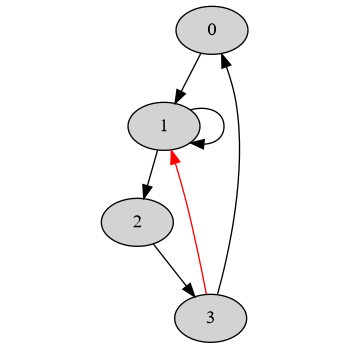
\includegraphics[width=.8\linewidth]{figures/GD_block}
\caption{Graph created from block-matrix, the highlighted edge is not well resolved by \ref{eqn:co} if $N_b^o \neq 0$}
\label{fig:GD_block}
\end{figure}

\begin{figure}%[!th]
\centering
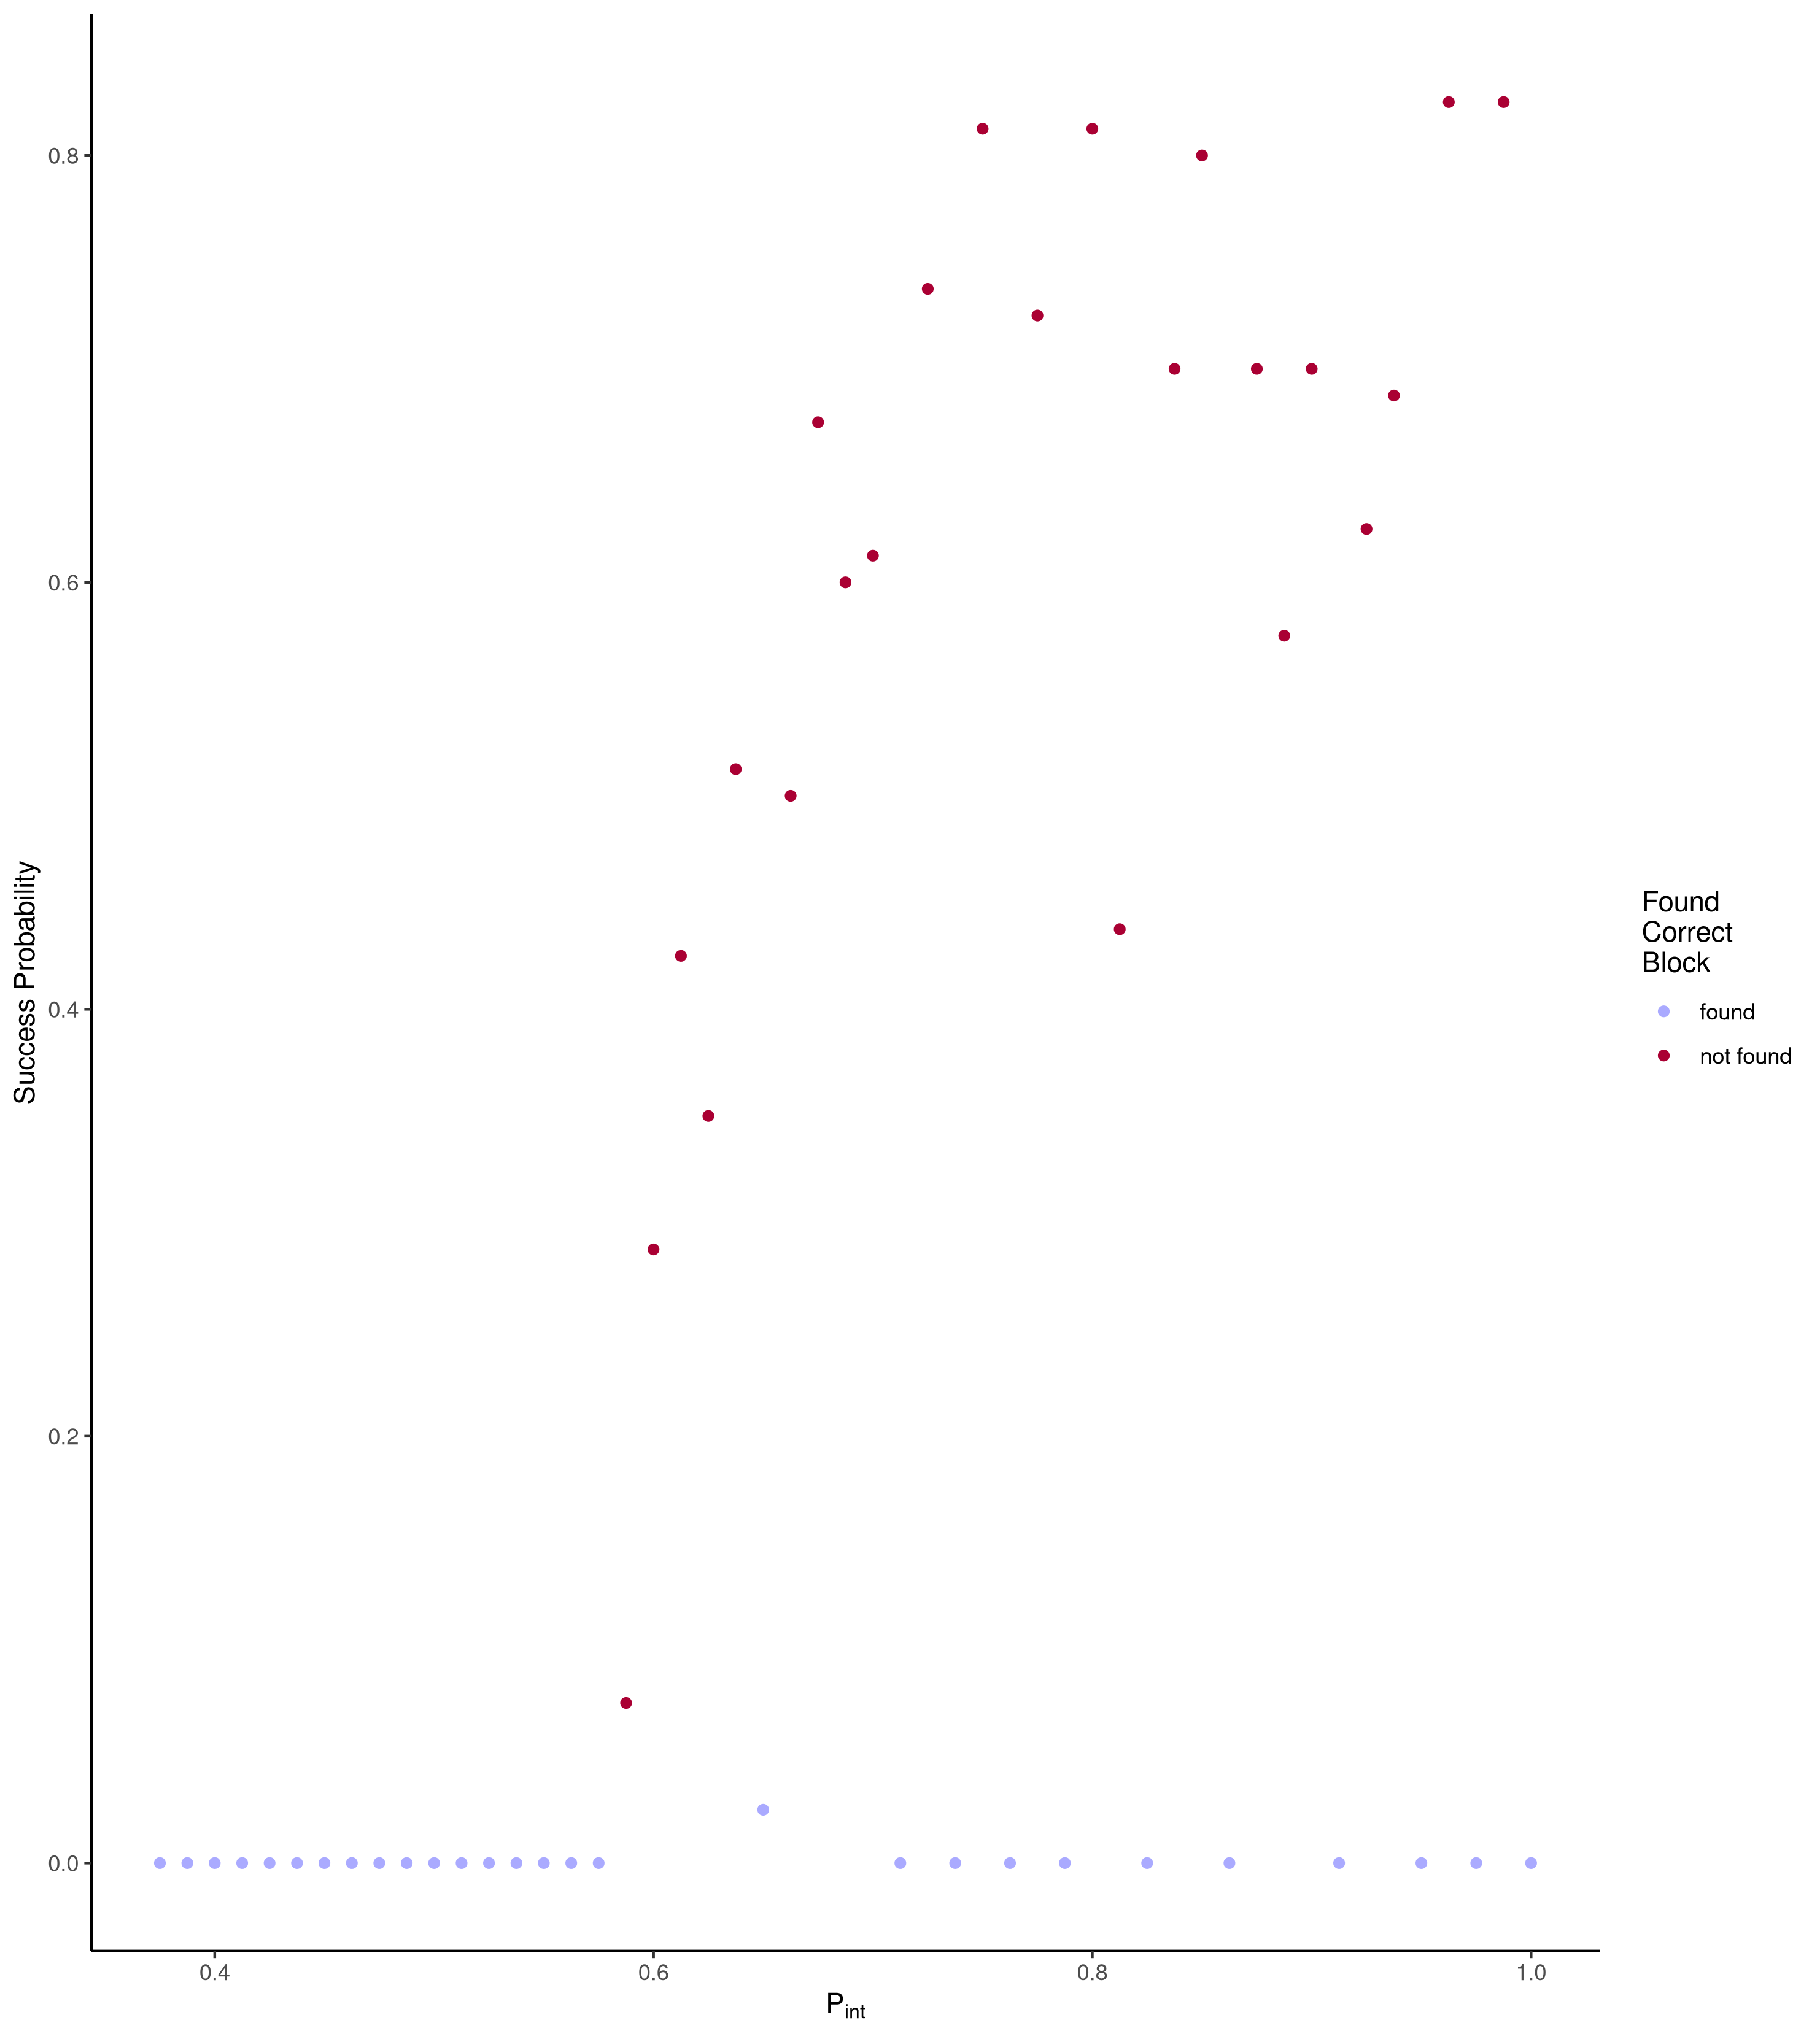
\includegraphics[width=.9\linewidth]{figures/GD_prob_fill}
\caption{The probability of finding the correct block for graphs with $N_b = 20$ and $N_b^o = 5$ per run of GD, for different values of $P_{int}$, while keeping the number of edges constant. The probability increases rapidly from $0$ to $0.4$ at $P_{int} \approx 0.6$. It keeps increasing until it is roughly constant above $p_{int}$ = 0.8. Another feature of the graph is showing whether the block-image found from the partition maximising \ref{eqn:co} converges to the correct block image, which is found to not be the case for half of the networks considered. }
\label{fig:GD_random_fill}
\end{figure}

\begin{figure}%[!h]
\centering
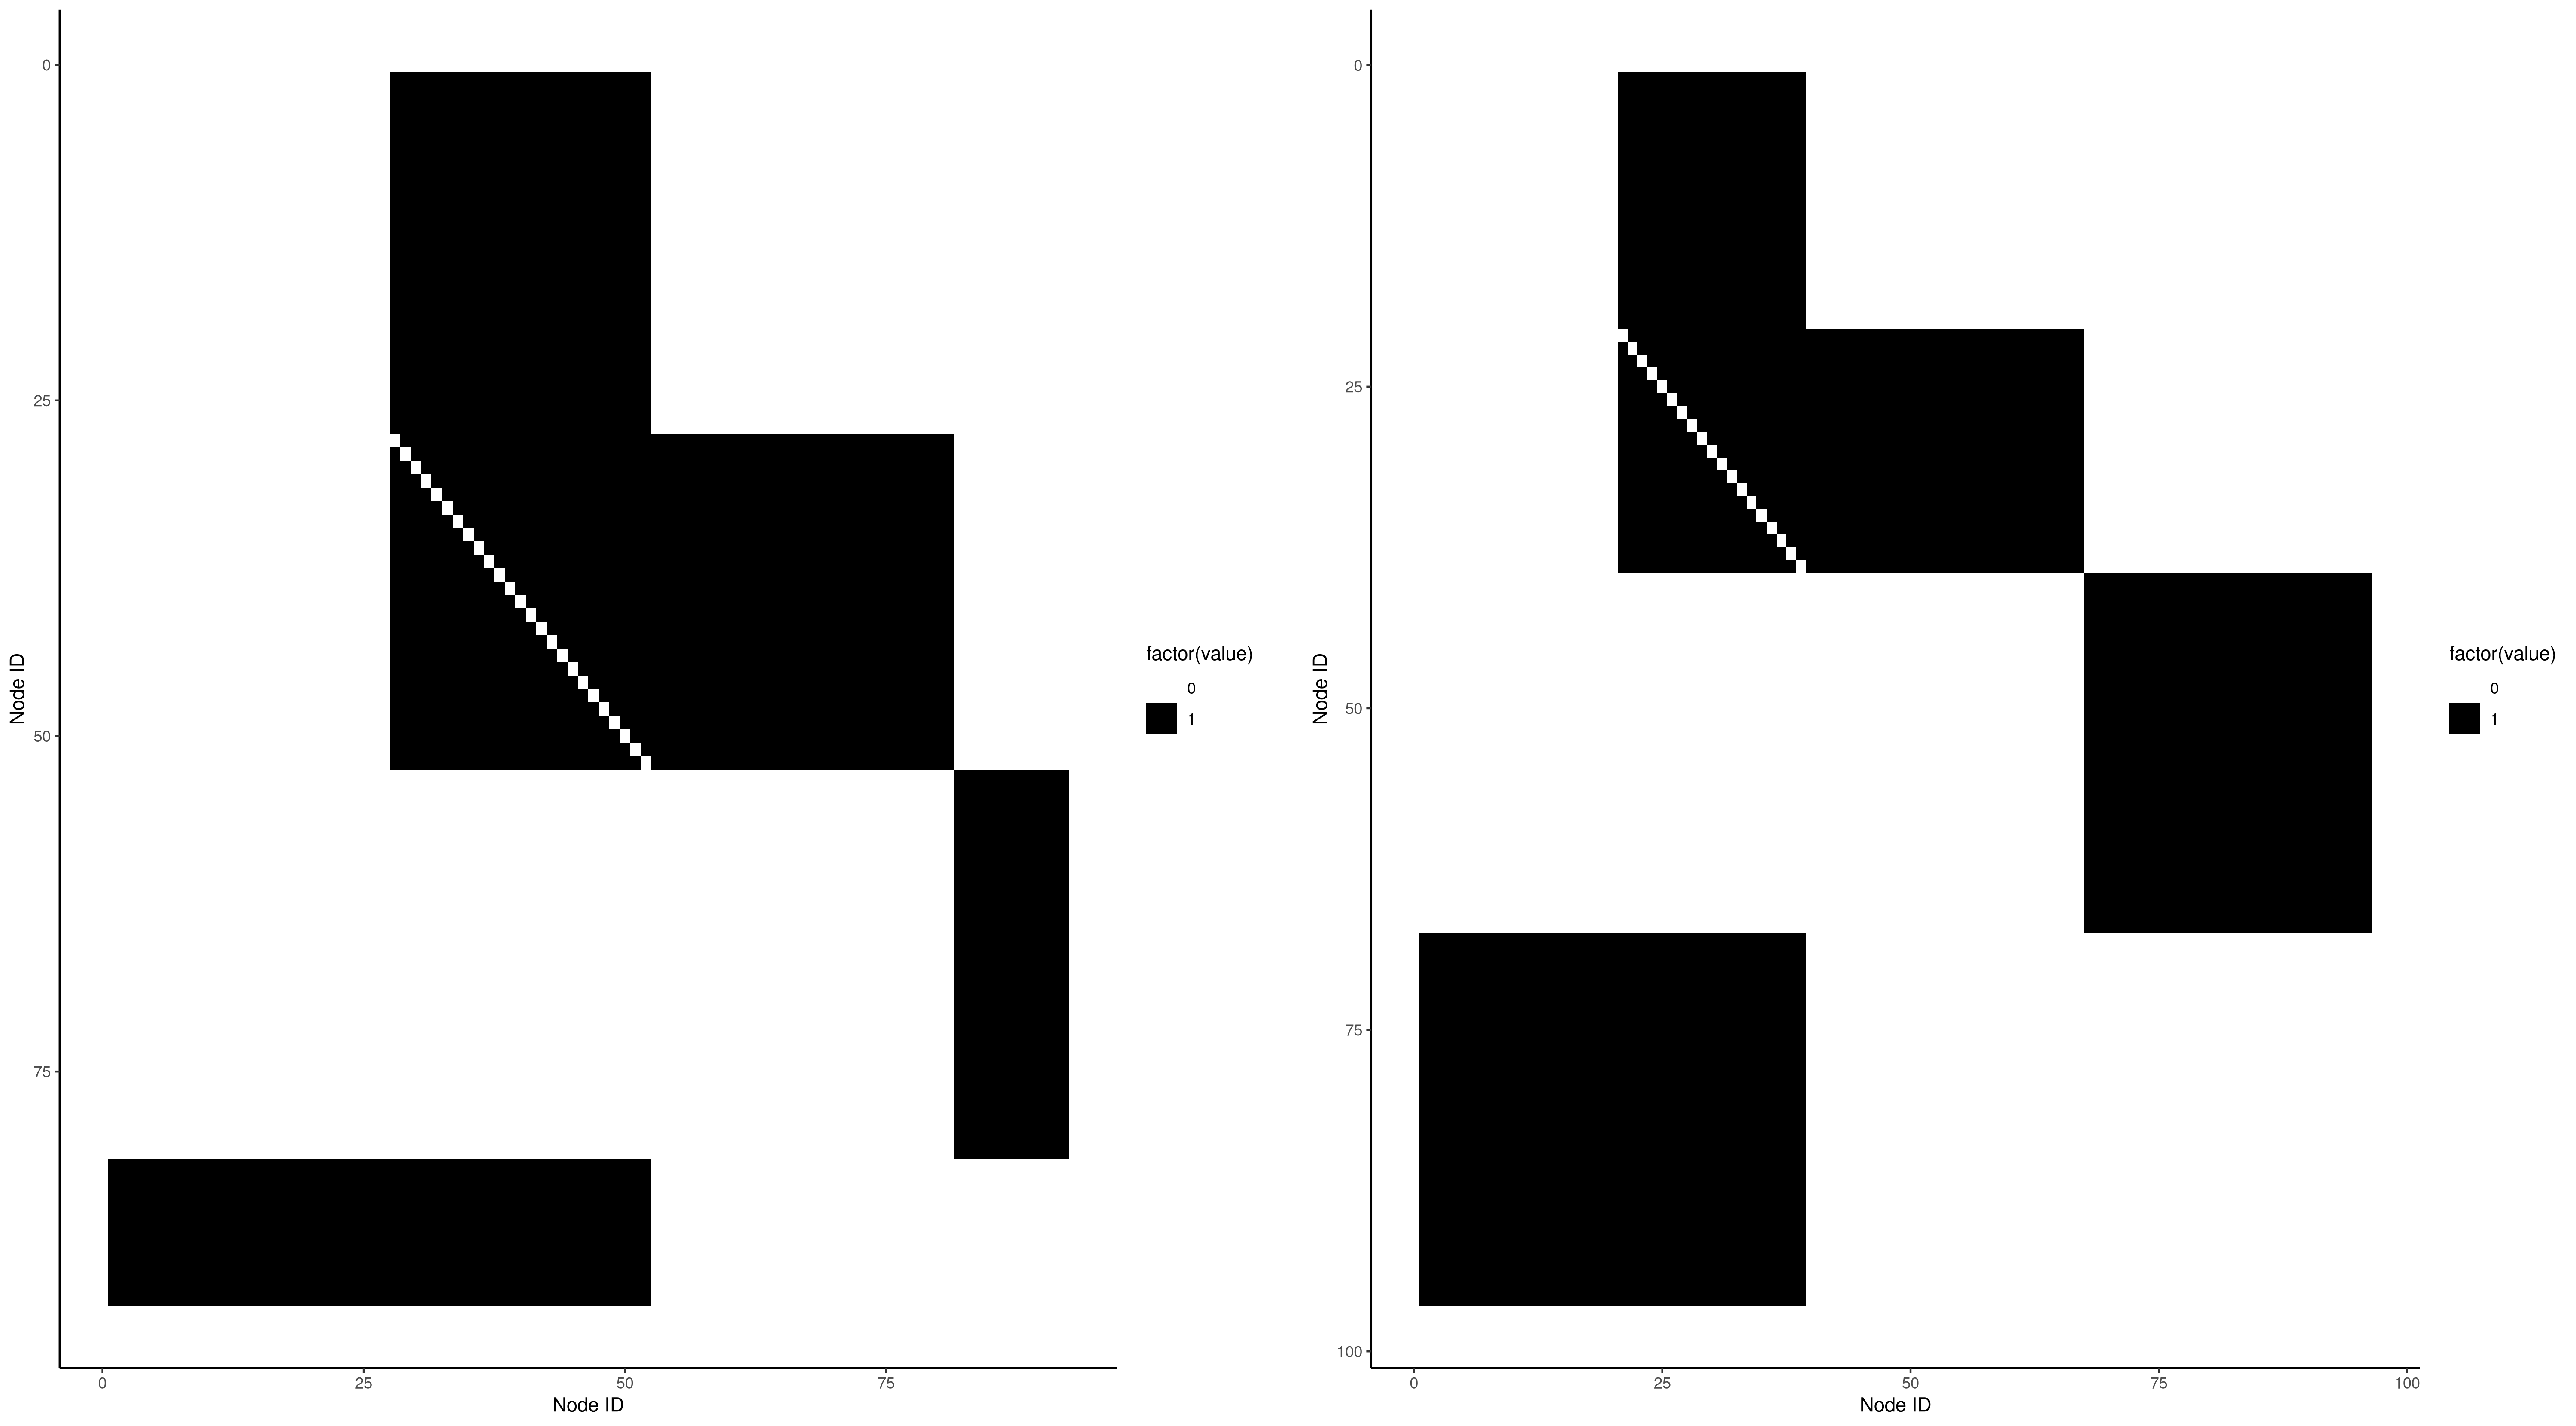
\includegraphics[width=.8\linewidth]{figures/block}
\caption{Adjacency matrices for two randomly chosen networks, colour represents value, with 1 being black and 0 white}
\label{fig:GD_adj}
\end{figure}

\begin{figure*}%[!h]
\centering
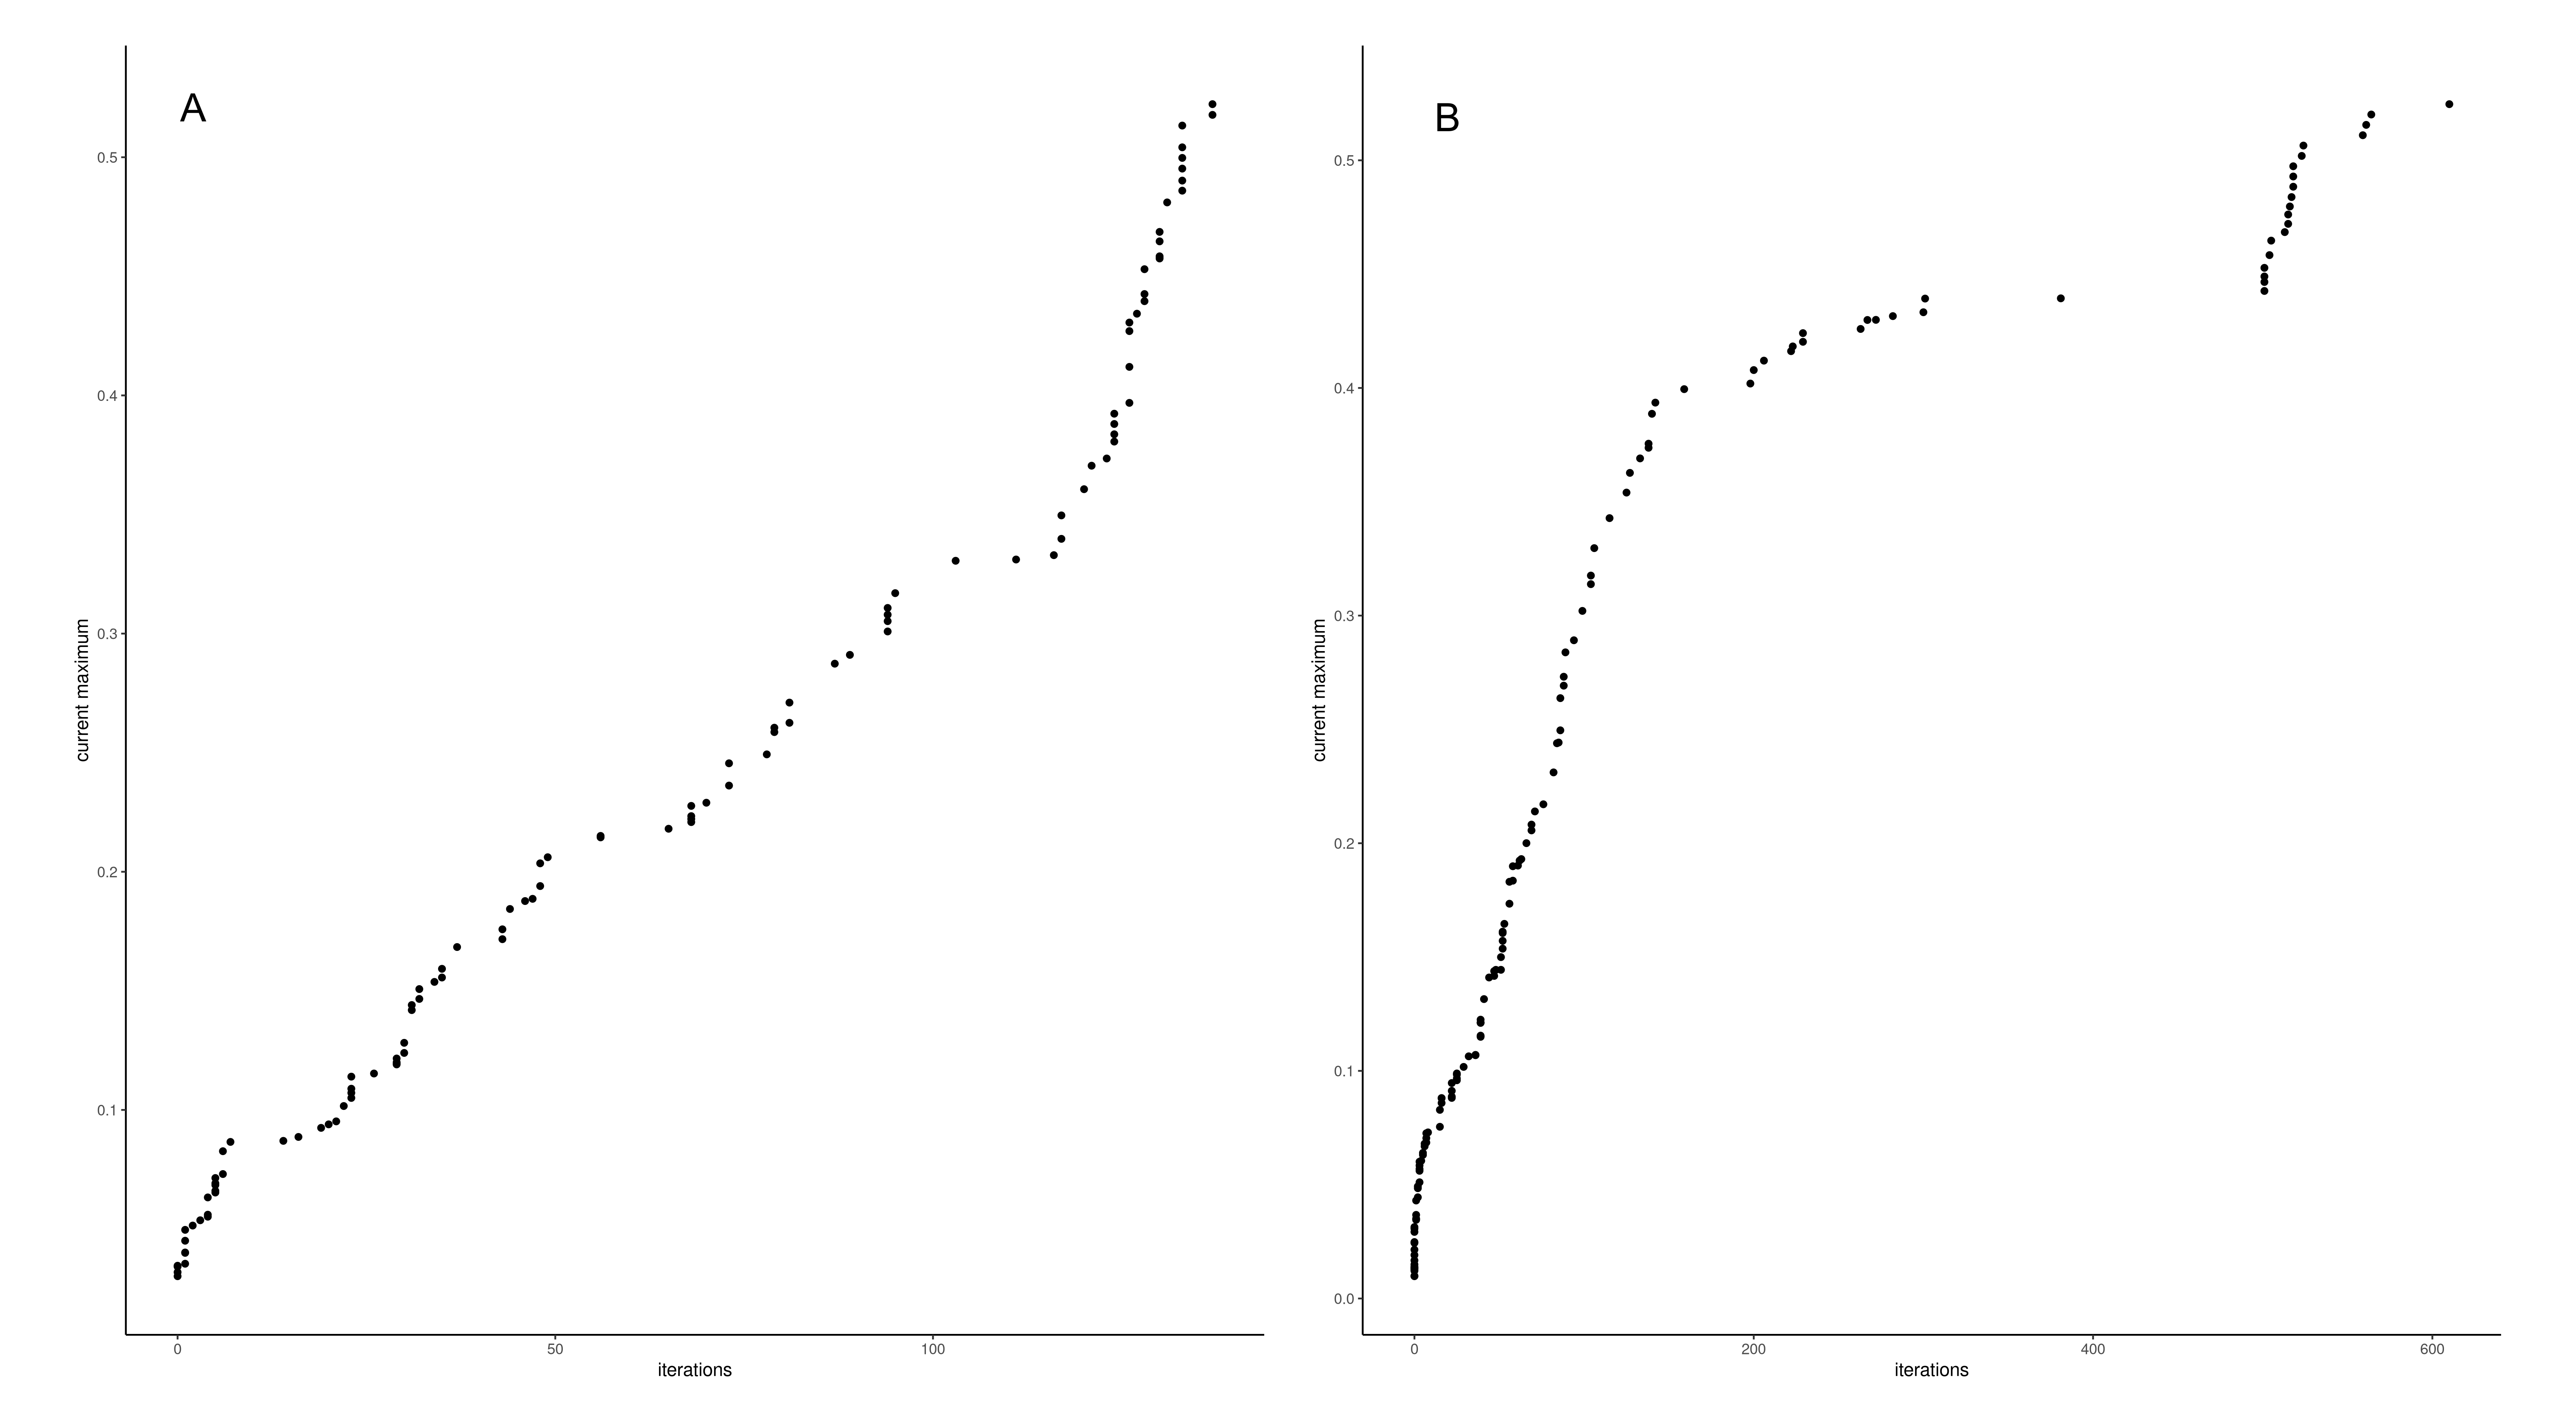
\includegraphics[width=.9\linewidth]{figures/SA_sched_comp}
\caption{Optimisation of a $N_b=20$,  $N_b^o=5$ network. $T_{max} = 3$ A) shows optimisation with an exponential annealing schedule $T_{t+1} = 0.95 T_{t}$. B) optimisation with a reciprocal annealing schedule $T_{t} = T_{max}({1 + t})^{-1}$. It can be seen that with an exponential annealing schedule, the rate of growth of the maximum is nearly linear, but with the reciprocal there is linear growth at the beginning, with a period of very little activity. This suggests that the temperature can be made to reduce at a faster rate}
\label{fig:SA_max_naive}
\end{figure*}

\begin{figure}%[h]
\centering
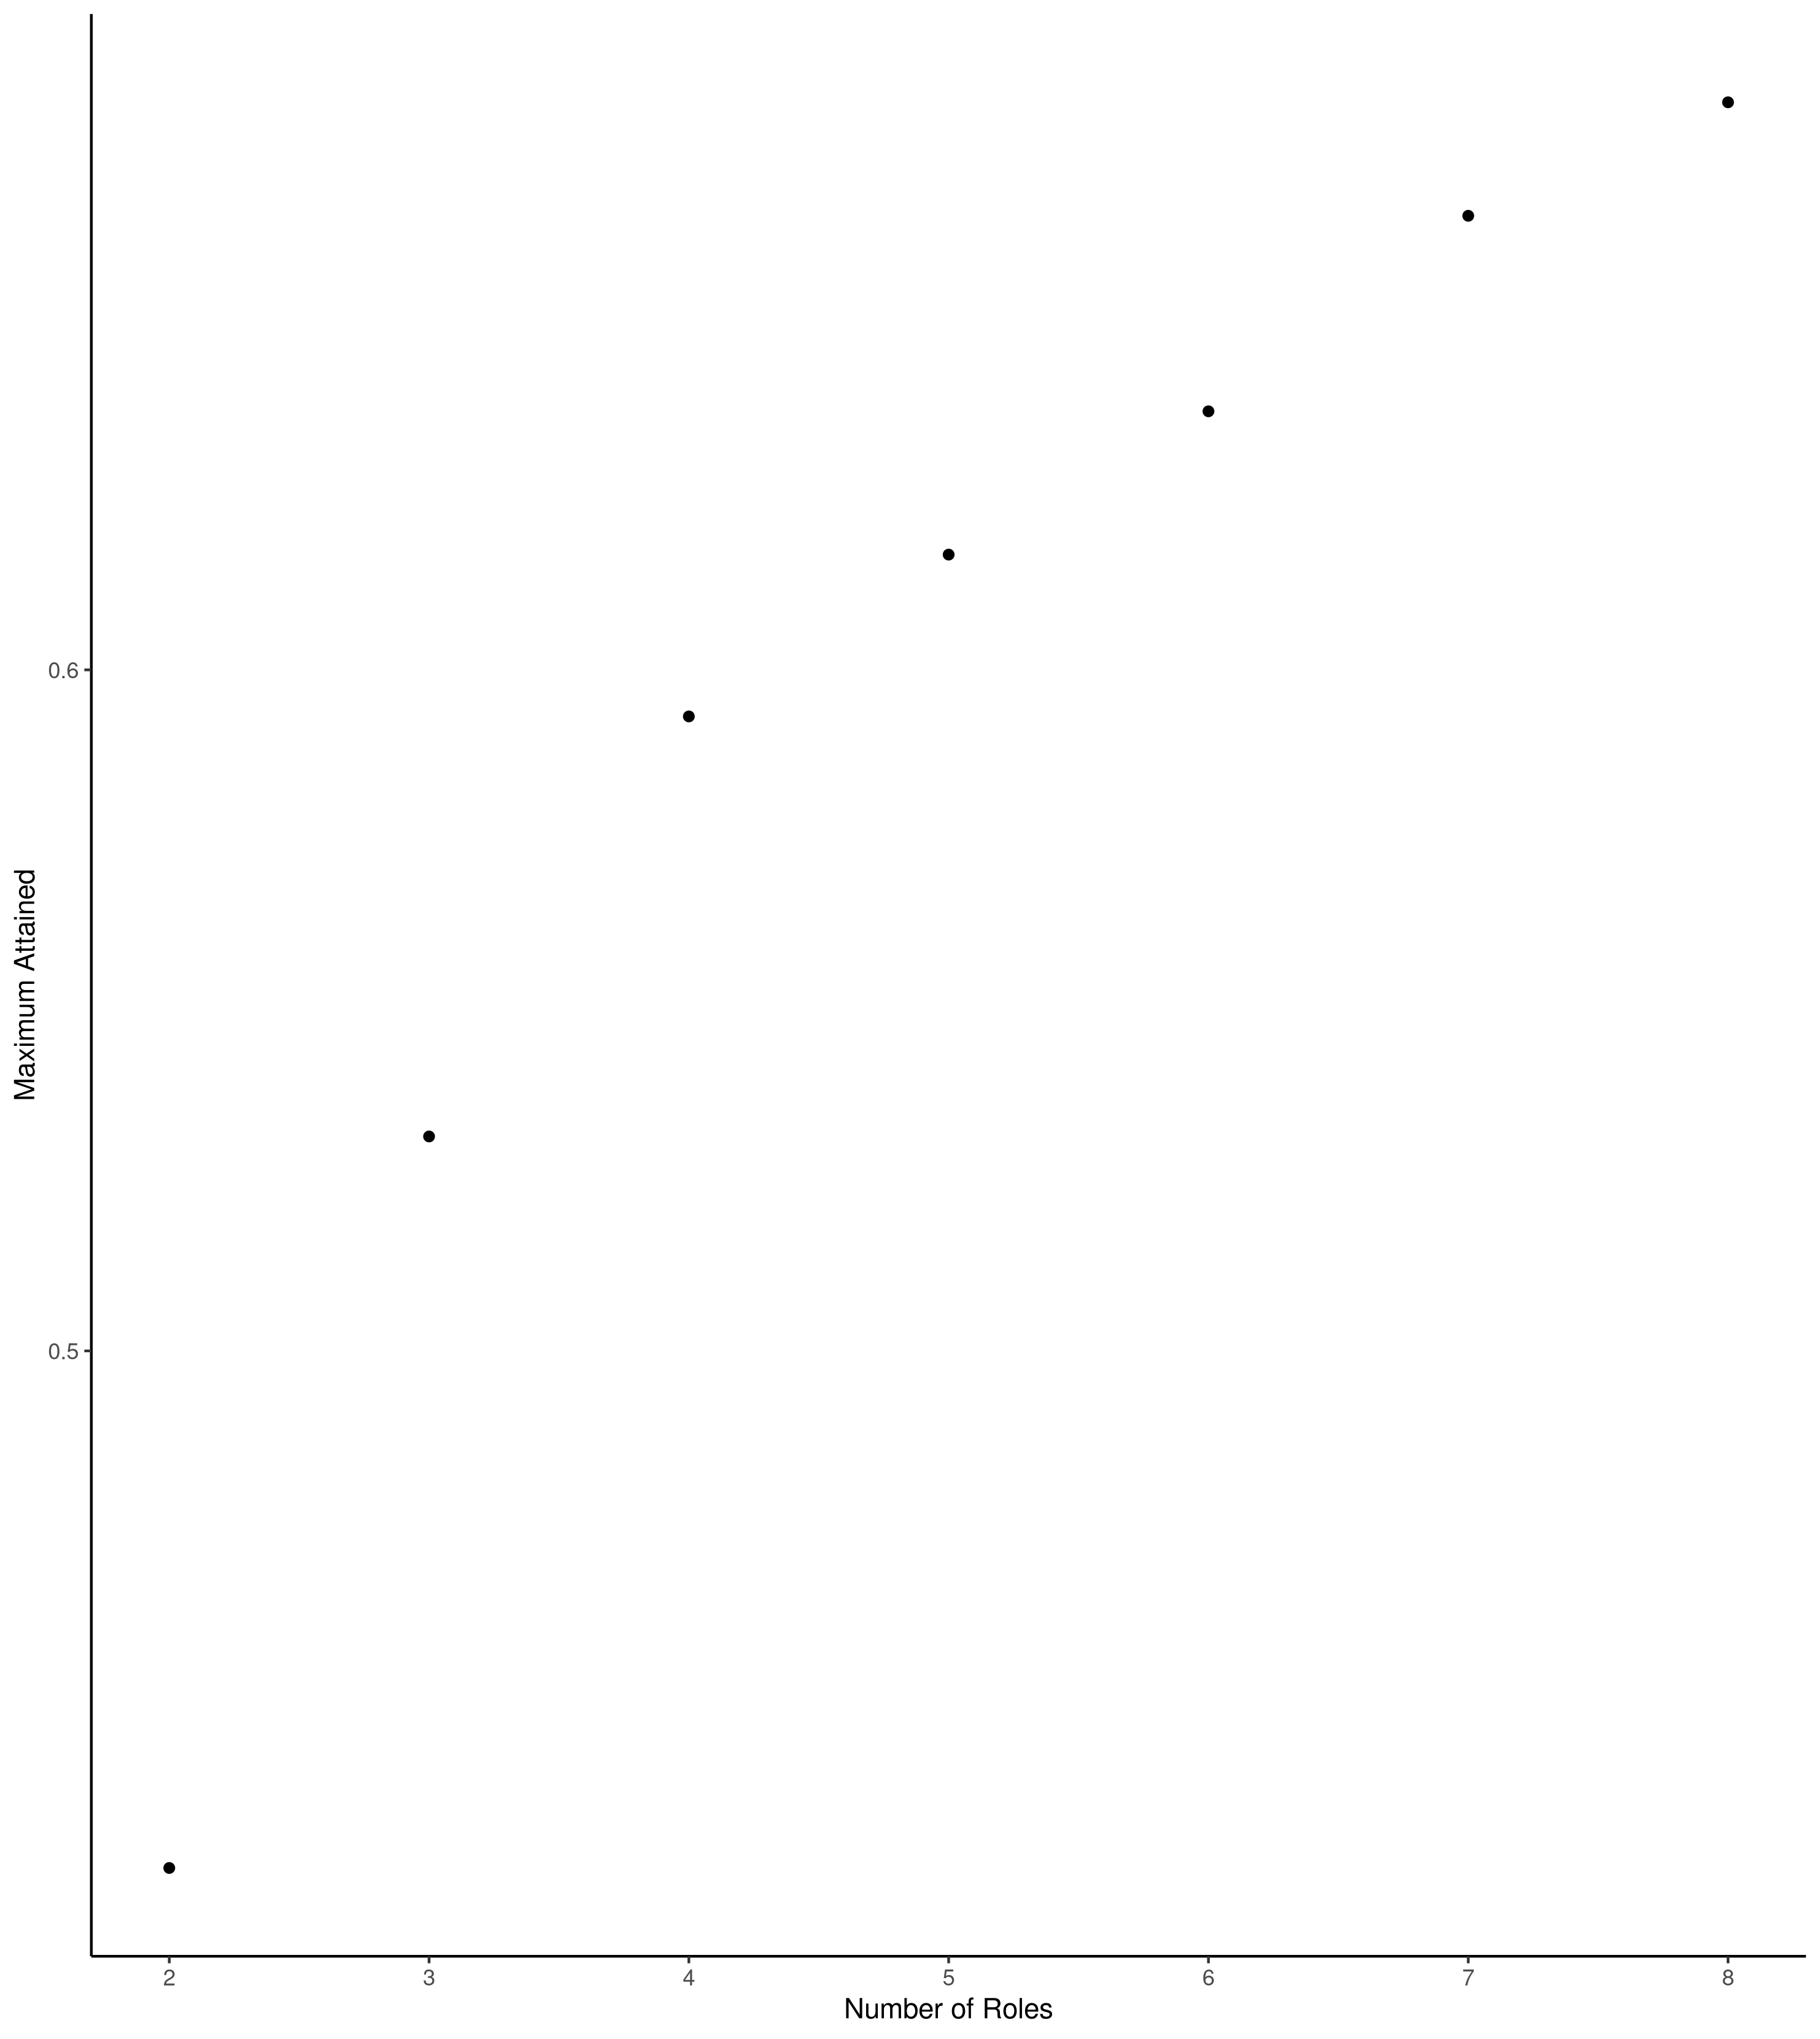
\includegraphics[width=.8\linewidth]{figures/prison_maxima_roles}
\caption{Partition Optimisation for Gagnon \& MacRae prison, showing a change to linear behaviour at $M =4$ the data was generated by running the SA optimisation algorithm and choosing the highest value with $R_i = 20N$ and  $T_{t + 1} = 0.95 T_t$}
\label{fig:roles}
\end{figure}


\begin{figure}%[h]
\centering
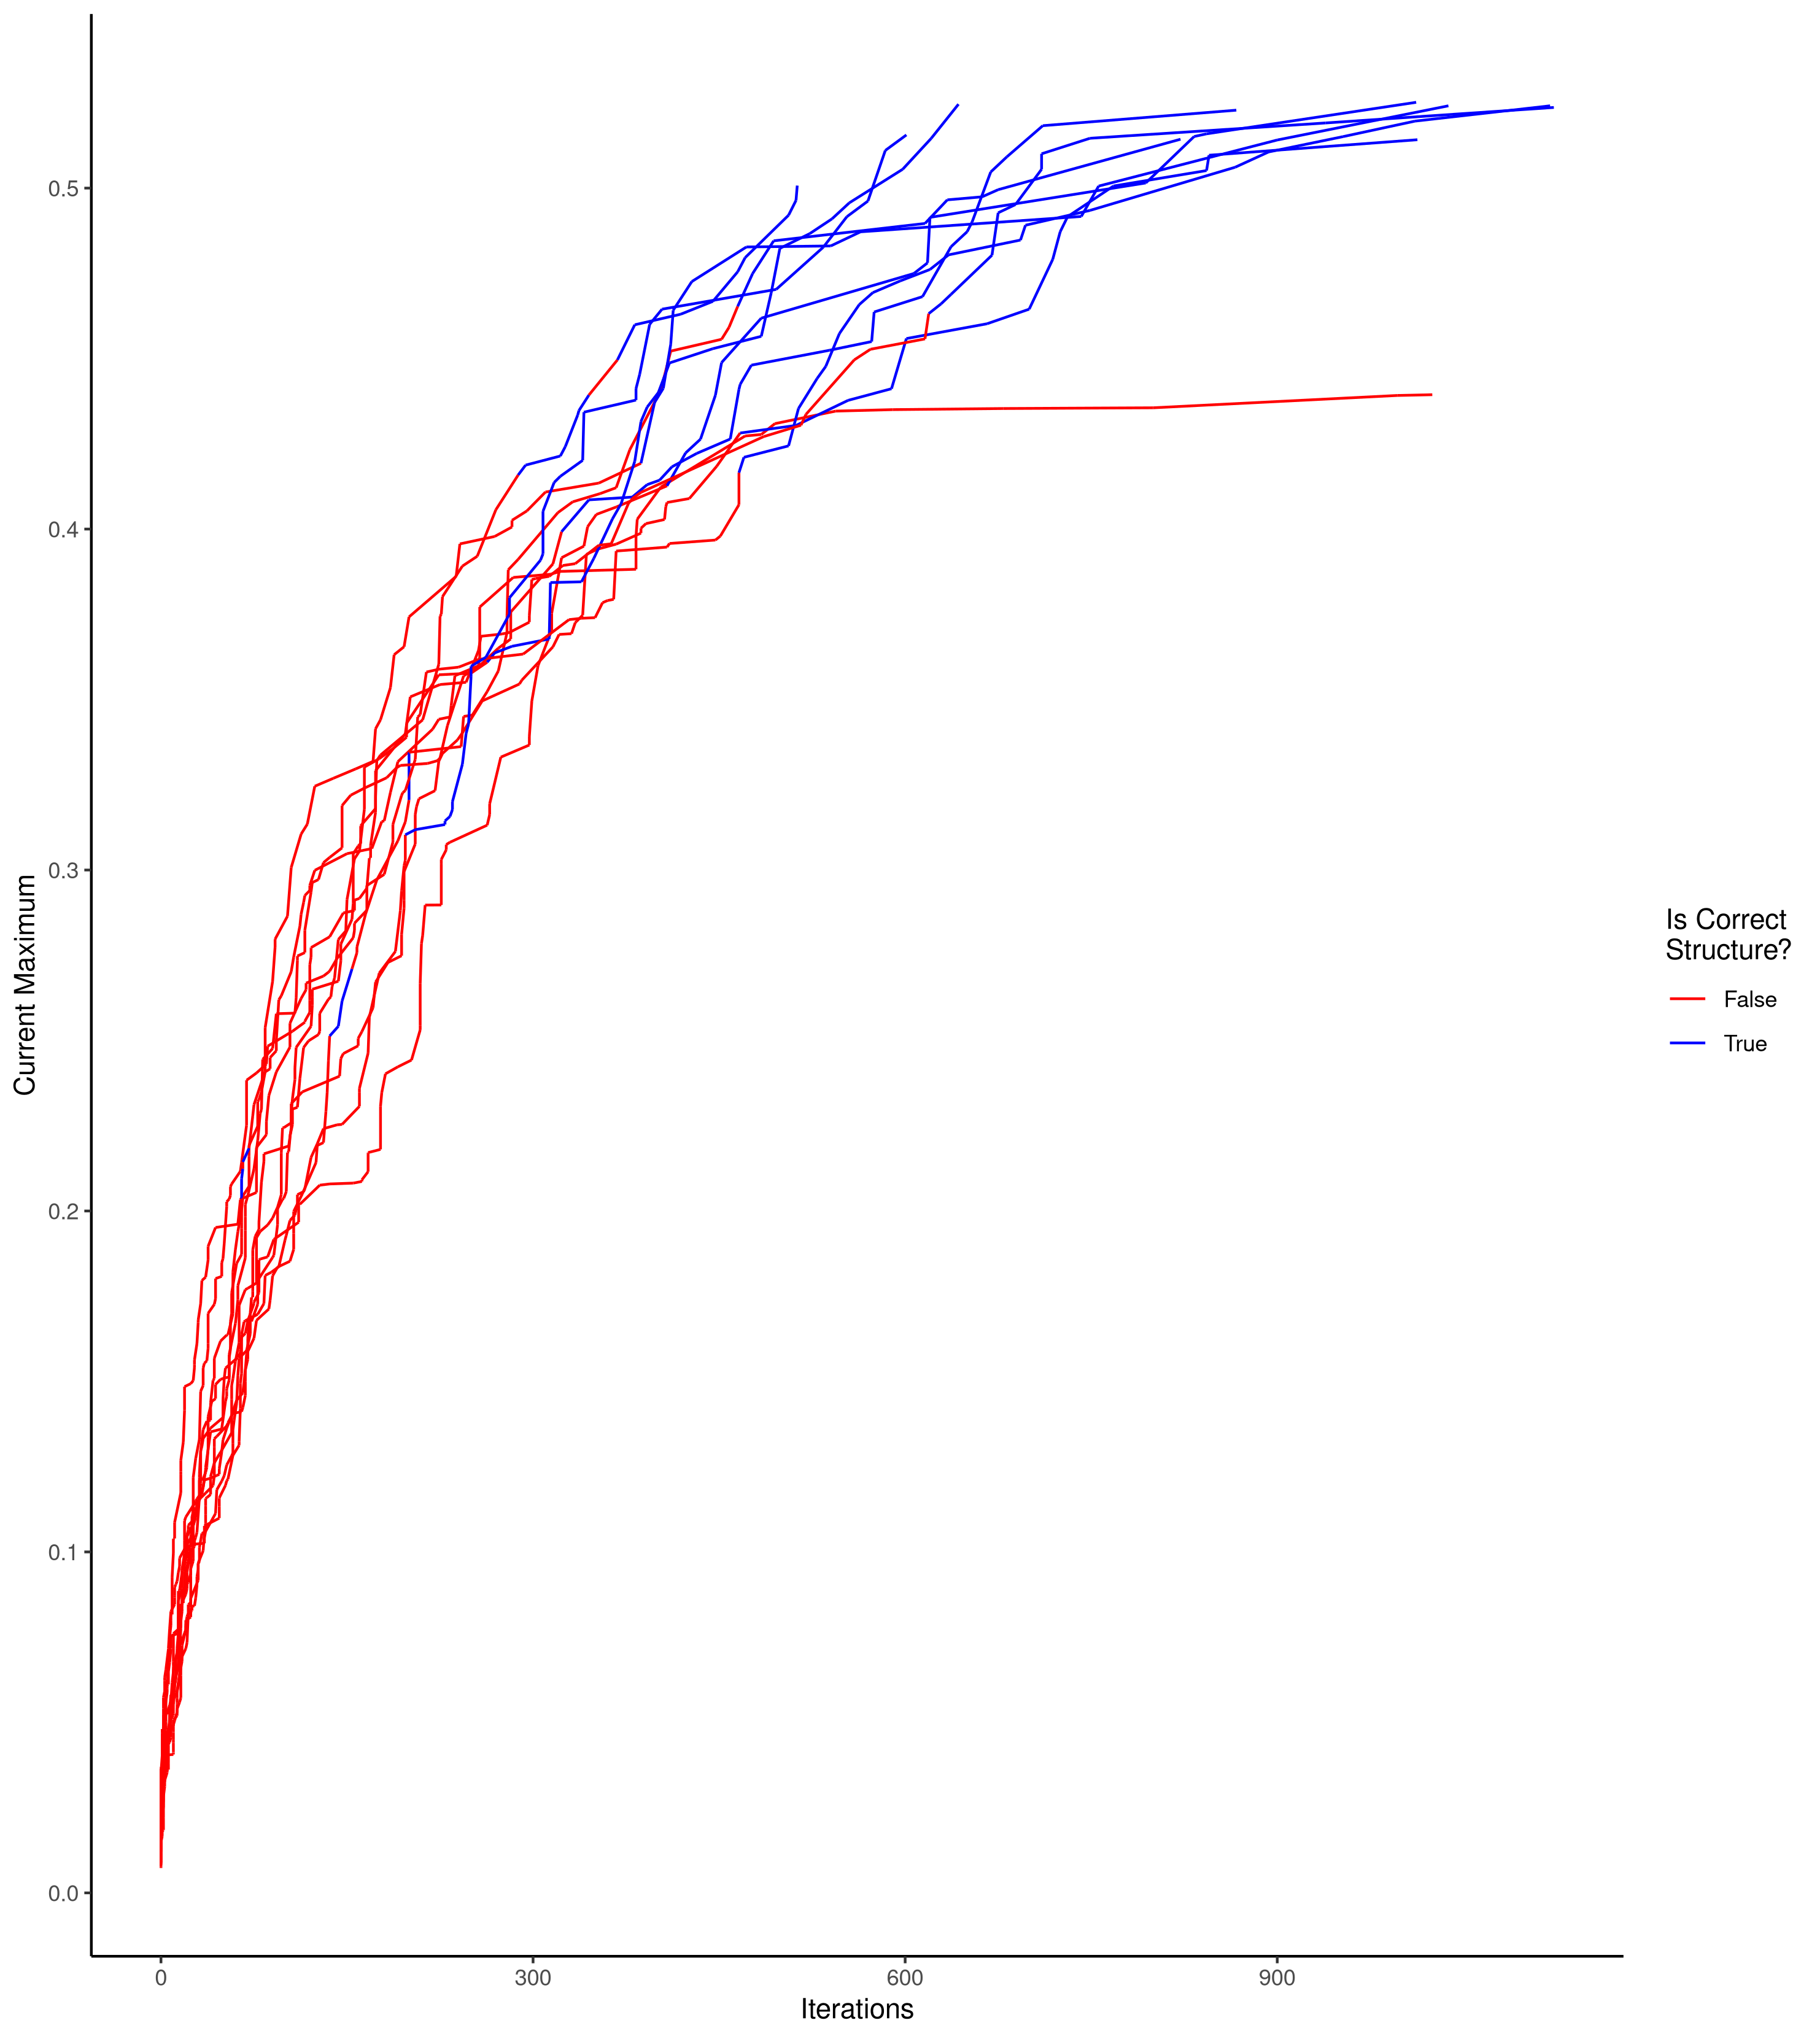
\includegraphics[width=.8\linewidth]{figures/multiple_runs}
\caption{Multiple runs of the algorithm, with only varying inital states. Most of these converge to the correct final block-image, but two don't. It can be clearly seen that the correct block image is achieved by the runs that achieve a high maximum.}
\label{fig:multiple_runs}
\end{figure}

\begin{figure}%[H]
\centering
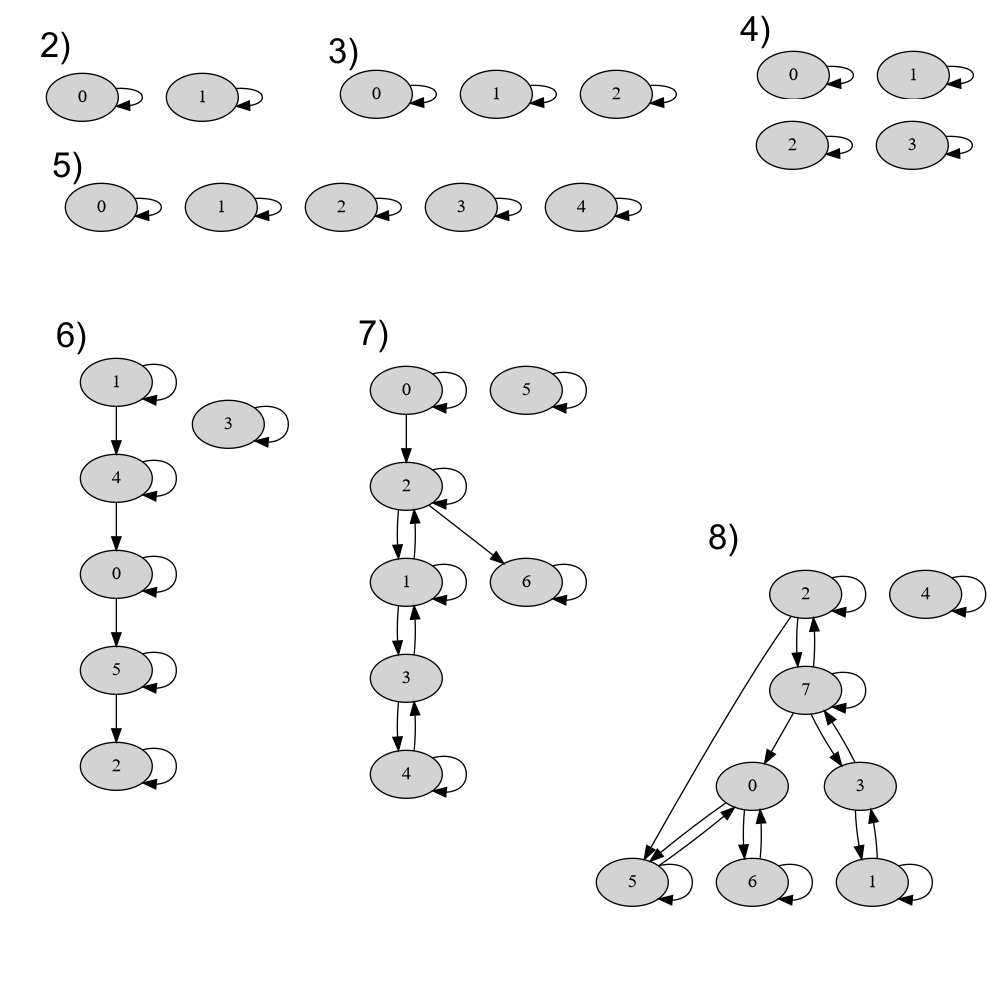
\includegraphics[width=.8\linewidth]{figures/blocks_prison}
\caption{Graphs of the block images for each of the roles calculated for the prison network. Up until $M=5$ the network no nodes are weakly connected, showing tightly-knit friendship groups between inmates. } 
\label{fig:prison}
\end{figure}

\subsection*{Analysis of Simulated Annealing}
As simulated annealing works by exploring the state-graph with random walks, we take $R_i$ to be a multiple of the diameter of the state-graph. This diameter is simply  $N$. In this article, the constant of proportionality we take is 4, so $R_i = 4N$ unless otherwise indicated. We analyse our implementation by applying it to networks generated by the previous section. Every time the algorithm finds a new maximum, we store the temperature it was found at, as well as the number of temperature iteratios, $t$. A specific run of this is shown in Fig. \ref{fig:SA_max_naive}. We also show multiple runs using the same network but with adjusted exponential scaling $\alpha = 0.999$, which can be seen in Fig. \ref{fig:multiple_runs}. 


\subsection*{Analysis of Prison Relationship}
We now present an analysis of the Gagnon \& MacRae prison dataset found in \cite{prison}. For this dataset 67 prison inmates were asked the question "What fellows on the tier are you closest with?" and each was free no choose as many friends as he desired. We determine the critical number of roles is given by $M = 4$, as shown in Fig. \ref{fig:roles}. At this number of roles, the block matrix is diagonal, meaning that the best role assignment specialises to Newman Modularity \cite{modularity}. This was in fact found to be the case for all values of  $M$ from 2 to 5. All of the block images are plotted in Fig. \ref{fig:prison}.  

\section*{Summary}
We have shown that both gradient descent and simulated annealing can be applied effectively to the problem of optimising functions on networks, and provided an efficient $O(N)$ way to calculate the differences in cost between state. SA suffers from dependence on initial conditions, but this can be mitigated by running the algorithm repeatedly and choosing the highest value, this option is costly but would assure that the global maximum, or a state close to it, is found. Unlike with SA, the only parameter we have for GD is the number of repetitions and it's difficult to decide when to stop the algorithm.    

\subsection*{Further Questions}
    The choice of neighbourhood of a state should depend on the algorithm used. The runtime of GD is linear in the size of the neighborhood. Large neighbourhoods would allow the sampling of a larger space per iteration, and would reduce the number of local maxima. An interesting avenue would be to plot the dependence of runtime to neighbourhood size to try find an optimum. SA would also benefit from this, but seemingly without the drawback of computational complexity. There also is the problem that more complicated state neighbourhoods would mean that updating $e_{rs}$ and $[e_{rs}]$ would no longer be  $O(N)$. \\The area of choosing the correct parameters for SA still needs more research, specifically the exponenial factor as well as the number of iterations at each temperature. As the state-graph is regular, perhaps walks could be treated as multidimensional random walks, and $R_i$ could be chosen analytically so that the walk has some fixed probability $p$ of ending up a distance equal to the diameter away from the sarting state. \\ 
Different methods of sampling with GD could be explored. For example, rather than randomly sampling nodes in the state-graph, sample them uniformly. Though, this approach would only work on small networks. An idea would be to use poisson-disk sampling, as distances in the state-graph can be calculated quickly. This would help create a more uniform sampling. 
\subsection*{Remarks On Originality}
All code is written by me and is available either at www.github.com/4Kamei/RoleOptimisation, or by directly contacting me by email. \\ 
Although the idea of calculating deltas isn't new, my approach applied to this specific problem is original. \\ 
The ideas behind simulated annealing and gradient descent have been around for a long time so they aren't novel, though the implementation of both of them is my own.
All plots were created with R using ggplot2 and reshape2 libraries. 
Code was written both in Java using Gson, as well as in Python utilising networkx and numpy. 
% Bibliography

\section*{References}

\bibliography{cite}

\end{document}
